\section{Decision Trees, Ensemble Approaches}
\begin{itemize}
	\item Decision trees are very powerful -- in instances where we can use decision trees to perform
		classification, they almost always outperform alternative methods.  
	\item One nice thing about decision trees is that you don't really have to go through the trouble of
		hyperparameter tuning, and they are also highly interpretable, unlike neural networks.   
	\item You can really think of these as a game of "20 questions", where you ask a bunch of yes or no
		questions and decide the classification based on the answers.   
	\item The nonlinearity offered by recursive decision boundaries is very powerful, and is something linear
		regression models cannot do.
	\item \comment{Some cons: the decision boundary is not smooth, and they are relatively unstable and
		sensitive to changes in the data.}
\end{itemize}

\subsection{Structure}
\begin{itemize}
	\item The goal is that given a set of "features" \( X \), if we can predict some other feature. For
		instance, given the horsepower, weight, maker of a car (\( X \)), we can be asked to predict the miles per
		gallon, \( Y \).
	\item Mathematically, we are essentially trying to learn a class of functions \( f: X \to Y \) where \( X
		\) is the features and \( Y \) are the possible outputs.    
	\item Before we look at how the decision tree is built, we look at how we use one. Given some input data,
		the decision tree determines the order in which we query the parameters to determine a result. These
		queries may not be the same length, as sometimes a single query is enough to determine a result.    

		Each node in the decision tree is essentially a query to an attribute \( x_i \), and depending on its
		value we follow the corresponding edge. Leaves in this tree correspond to the classifications \( y
		\).  
	\item Compared to linear models like KNNs, decision tree boundaries \textit{must} be axis-aligned. This
		is an issue, because it means that the decision boundary is usually more complex than linear
		regression models, or it would take more information to replicate the same boundary.  
	\item Another benefit of decision trees is that because they can grow arbitrarily large, its limit is
		basically a truth table, so this means that you can represent any function of the input attributes
		with a decision tree.     
\end{itemize}

\subsection{Building Decision Trees}
\begin{itemize}
	\item To start, the simplest decision tree we make is one which doesn't consider the data at all, and
		just classifies all data based on the \( y \) that is most common in the training data. Obviously
		this is not interesting, so we move on. 
	\item Then, you look at a single feature, and create a node for every possible value that the feature
		could take on. Then for each of these values, find the \( y \) that is the most common, and that
		becomes your prediction.
		\begin{center}
			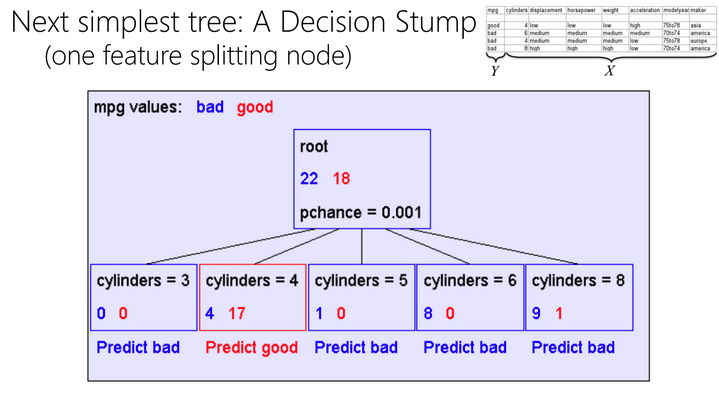
\includegraphics[scale=0.5]{images/lec17-1.png}
		\end{center}
		So here we first query on the number of cylinders, then based on the majority mpg (either good or
		bad) in each cylinder category we can come up with a classification that makes sense. We then
		recursively do this, and find the next best query to look at. This will be different for different
		nodes:  
		\begin{center}
			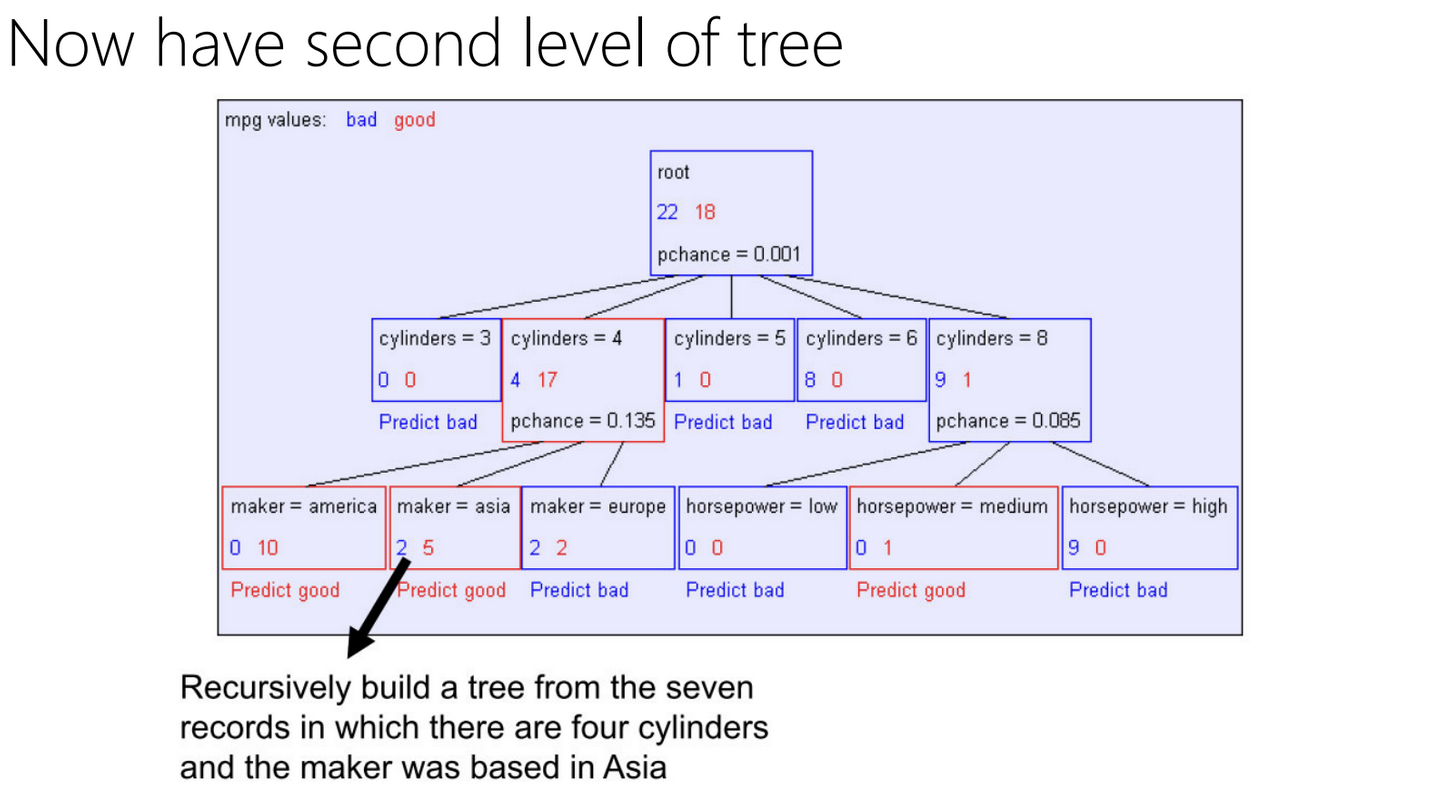
\includegraphics[scale=0.5]{images/lec17-2.png}
		\end{center}
	\item So how do we grow this tree? What feature do we split on? The goal is to make leaf nodes to be
		pure (consisting of only one class), so we want splits which increases the purity of the leaf nodes.  

		One way to quantify this purity is to quantify how surprised we are at seeing a particular result,
		and then compute the \textit{entropy}, which is the expected surprise overall. The entropy is defined
		as:
		\[
			H(Y) = -\sum_k P(Y = k) \log P(Y = k)
		\]
		The negative is there to signify the fact that rare events are more entropic than common ones. Pure
		nodes which don't have misclassifications have zero surprise, so finding the best split is the same
		as finding the classification which minimizes entropy.    
	\item Thinking of distributions more generally, high entropy tend to spread their mass over the entire
		space, whereas low entropy generally has its probability mass concentrated at a particular point.   
	\item In the training data, we can't compute teh entroyp of \( Y \), but we can control the entropy of \(
		p(Y \mid X)\), since we control the feature \( X \) that we want to look at. So, our goal is to
		reduce the \textit{conditional entropy} at each node so that we eventually reach a surprise of zero. 

		The conditional entropy is just given by:
		\[
			H(Y \mid X_{j, v}) = P(X_{j, v} = 1) H(Y \mid X_{j, v} = 1) + P(X_{j, v} = 0) H(Y \mid X_{j, v} =
			0)
		\]
		By the rules of expectation, this conclusion should be relatively obvious. Here \( X_{j, v} \) is a
		binary random variable, so we only have two terms, but you can imagine a case where we have more. The
		point here is that we split on the values that \( X_{j, v} \) could equal, then compute the entropy
		for each subcategory and weight them accordingly.   

		\comment{Some books use the base-2 logarithm here; it makes no difference versus base-10 log.}  
	\item Equivalently, we can phrase this as maximizing the \textit{information gain}, which is defined as:
		\[
			I(X_{j, v}; Y) := H(Y) - H(Y \mid X_{j, v})
		\]
		\( H(Y) \) is the entropy you start with (constant), and compute the conditional entropy for the
		different \( X_{j, v} \) labels and maximize this quantity.   

		\comment{There are no parameters and "learning" here! This is really just chugging through to find
			best possible feature to split on. For real valued features, you pick a threshold to split on
		instead.}
	\item When do you stop recursing on a node? There are two cases:
		\begin{enumerate}[label=\arabic*.]
			\item If the category \( Y \) is pure after the classification, so all results after sorting are
				of a single class.
			\item If the remaining features to split on don't improve the data at all, then the node becomes
				unexpandable. Note, this is not the same as zero information gain. In cases like these, you
				just flip a coin to decide how to predict. 

				\question{In the slides, they write this as "all input values are the same", how is the
					lack of further classification (or lack of improvement) related to the fact that all
					input values are the same? Couldn't you just have a 1-1 tie with the input values not being the
				same?} 
		\end{enumerate}
\end{itemize}

